\documentclass[fleqn]{article}

\usepackage{amsmath} % for equations
\usepackage{amssymb} % for symbols
\usepackage[margin=0.75in]{geometry} % for setting margin
\usepackage{tikz} % for drawing
%\usepackage{verbatim} % for multiline comments
\usepackage{graphicx} % for pics
\usepackage{parskip} % looks nice
\usepackage{scrextend} % for block indentation

\title{Assignment 5}
\author{Raz Reed}
\date{October 2, 2017}

\begin{document}
\pagenumbering{gobble}
\maketitle

\newpage
{\Large\bf Problem 8.11}\vspace{1em}\par
\textbf{(a)} An RBT is recursively defined:
\begin{enumerate}
	\item The empty tree $\varepsilon$ is an RBT.
	\item If $T_1,T_2$ are disjoint RBTs with roots $r_1$ and $r_2$, then linking $r_1$ and $r_2$ to a new root $r$ gives a new RBT with root $r$.
\end{enumerate}
Using this definition:
\begin{itemize}
	\item The first diagram is an RBT.\\
		  The empty tree $\varepsilon$ is an RBT $\rightarrow$ a root node with no children is an RBT $\rightarrow$ a root node with one left child and no right child is an RBT $\rightarrow$ a root node with one left child with two children is an RBT\par
	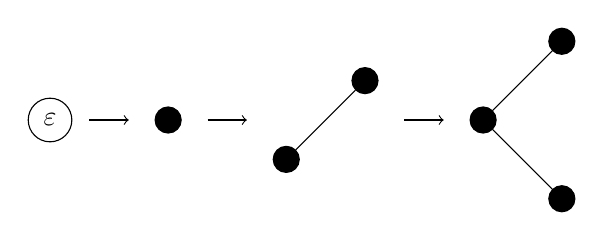
\begin{tikzpicture}
		\node [shape=circle,draw=black,fill=white] (A1) at (0.5,0) {$\varepsilon$};
		\draw [->] (1,0) -- (1.5,0);
		\node [shape=circle,draw=black,fill=black] (A2) at (2,0) {};
		\draw [->] (2.5,0) -- (3,0);
		\node [shape=circle,draw=black,fill=black] (A3) at (3.5,-0.5) {};
		\node [shape=circle,draw=black,fill=black] (B3) at (4.5,0.5) {};
		\draw (A3) -- (B3);
		\draw [->] (5,0) -- (5.5,0);
		\node [shape=circle,draw=black,fill=black] (A4) at (7,1) {};
		\node [shape=circle,draw=black,fill=black] (B4) at (6,0) {};
		\node [shape=circle,draw=black,fill=black] (C4) at (7,-1) {};
		\draw (A4) -- (B4);
		\draw (B4) -- (C4);
	\end{tikzpicture}
	\item The second diagram is an RBT.\\
		  The empty tree $\varepsilon$ is an RBT $\rightarrow$ a root node with no children is an RBT $\rightarrow$ a root node with two children is an RBT $\rightarrow$ a root node with two children whose left child has two children is an RBT\par
	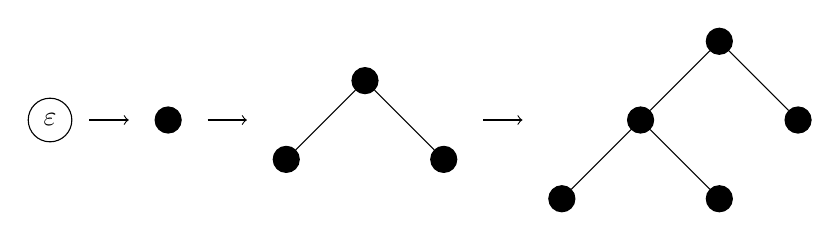
\begin{tikzpicture}
		\node [shape=circle,draw=black,fill=white] (A1) at (0.5,0) {$\varepsilon$};
		\draw [->] (1,0) -- (1.5,0);
		\node [shape=circle,draw=black,fill=black] (A2) at (2,0) {};
		\draw [->] (2.5,0) -- (3,0);
		\node [shape=circle,draw=black,fill=black] (A3) at (3.5,-0.5) {};
		\node [shape=circle,draw=black,fill=black] (B3) at (4.5,0.5) {};
		\node [shape=circle,draw=black,fill=black] (C3) at (5.5,-0.5) {};
		\draw (A3) -- (B3);
		\draw (B3) -- (C3);
		\draw [->] (6,0) -- (6.5,0);
		\node [shape=circle,draw=black,fill=black] (A4) at (9,1) {};
		\node [shape=circle,draw=black,fill=black] (B4) at (8,0) {};
		\node [shape=circle,draw=black,fill=black] (C4) at (10,0) {};
		\node [shape=circle,draw=black,fill=black] (D4) at (7,-1) {};
		\node [shape=circle,draw=black,fill=black] (E4) at (9,-1) {};
		\draw (A4) -- (B4);
		\draw (A4) -- (C4);
		\draw (B4) -- (D4);
		\draw (B4) -- (E4);
	\end{tikzpicture}
	\item The third diagram is not an RBT.\\Every RBT with $n \geq 1$ nodes has $n-1$ links. The tree in the third diagram has 5 nodes and 5 links, therefore it is not an RBT.
	\item The fourth diagram is an RBT.\\
		  The empty tree $\varepsilon$ is an RBT $\rightarrow$ a root node with no children is an RBT $\rightarrow$ a root node with two children is an RBT $\rightarrow$ a root node with two children and one left child is an RBT\par
	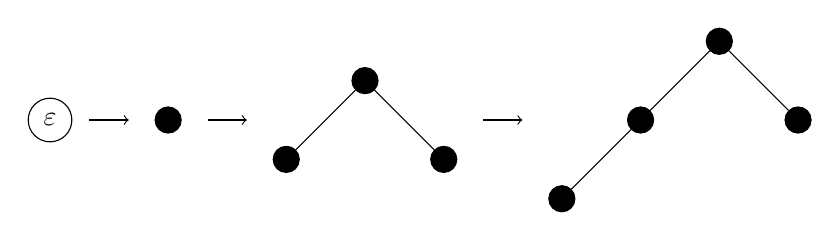
\begin{tikzpicture}
		\node [shape=circle,draw=black,fill=white] (A1) at (0.5,0) {$\varepsilon$};
		\draw [->] (1,0) -- (1.5,0);
		\node [shape=circle,draw=black,fill=black] (A2) at (2,0) {};
		\draw [->] (2.5,0) -- (3,0);
		\node [shape=circle,draw=black,fill=black] (A3) at (3.5,-0.5) {};
		\node [shape=circle,draw=black,fill=black] (B3) at (4.5,0.5) {};
		\node [shape=circle,draw=black,fill=black] (C3) at (5.5,-0.5) {};
		\draw (A3) -- (B3);
		\draw (B3) -- (C3);
		\draw [->] (6,0) -- (6.5,0);
		\node [shape=circle,draw=black,fill=black] (A4) at (9,1) {};
		\node [shape=circle,draw=black,fill=black] (B4) at (8,0) {};
		\node [shape=circle,draw=black,fill=black] (C4) at (10,0) {};
		\node [shape=circle,draw=black,fill=black] (D4) at (7,-1) {};
		\draw (A4) -- (B4);
		\draw (A4) -- (C4);
		\draw (B4) -- (D4);
	\end{tikzpicture}
\end{itemize}
Only the first, second, and fourth diagrams are RBTs.\\\par
\textbf{(b)} An RBT is an RFBT if and only if each node in the tree either has no children or has two.
\begin{itemize}
	\item The first diagram is an RBT, but has a node with one child. Therefore it is not an RFBT.\par
	\item In the second diagram, every node in the tree has either no children or has two, therefore it is an RFBT.\par
	\item The third diagram is not an RBT, therefore it is not an RFBT.\par
	\item The fourth diagram is an RBT, but has a node with one child. Therefore it is not an RFBT.\par
\end{itemize}
Only the second diagram is an RFBT.

\newpage
{\Large\bf Problem 9.2}\vspace{1em}\par
\textbf{(g)}
\begin{align*}
	\sum_{i=0}^{n}\left(\sum_{j=0}^{i} 2^i \right) &= \sum_{i=0}^{n}\left(\left(i+1\right)*2^i \right)\\
	&=\sum_{i=0}^{n}\left(i2^i\right)+\sum_{i=0}^{n}\left(2^i\right)\\
	&=\sum_{i=0}^{n}\left(i2^i\right)+2^{n+1}-1\\
	\\
	S(n)&=\sum_{i=0}^{n}\left(i2^i\right)\\
	S(n)&=1 \cdot 2^1 + 2 \cdot 2^2 + 3 \cdot 2^4 + ... + n2^n\\
	2S(n)&=2 \cdot 1 \cdot 2^1 + 2 \cdot 2 \cdot 2^2 + 2 \cdot 3 \cdot 2^3 + ... + 2(n-1)2^{n-1} + 2n2^n\\
	&=1 \cdot 2^2 + 2 \cdot 2^3 + 3 \cdot 2^4 + ... + (n-1)2^n + n2^{n+1}\\
	S(n)&=2S(n)-S(n)\\
	&=\qquad\quad\:\: 1 \cdot 2^2 + 2 \cdot 2^3 + 3 \cdot 2^4 + ... + (n-1)2^n + n2^{n+1}\ -\\
	&\quad\ 1 \cdot 2^1 + 2 \cdot 2^2 + 3 \cdot 2^3 + 4 \cdot 2^4 + ... + n2^n\\
	&=-2^1-2^2-2^3-2^4-...-2^n+n2^{n+1}\\
	&=n2^{n+1}-\sum_{i=1}^{n}2^i\\
	&=n2^{n+1}-\sum_{i=0}^{n}2^i+1\\
	&=n2^{n+1}-\left(2^{n+1}-1\right)+1\\
	&=n2^{n+1}-2^{n+1}+1+1\\
	&=2^{n+1}(n-1)+2\\
	\\
	\sum_{i=0}^{n}\left(\sum_{j=0}^{i} 2^i \right) &= \left(2^{n+1}(n-1)+2\right)+\left(2^{n+1}-1\right)\\
	&=n2^{n+1}+1
\end{align*}

\newpage
{\Large\bf Problem 6.19}\vspace{1em}\par
\textbf{(a)} Unstacking 4 boxes:\par
Method 1:
\begin{align*}
	&4 \rightarrow &\\
	&2,2 \rightarrow &\$4\\
	&1,1\ \ 2 \rightarrow &\$1\\
	&1,1\ \ 1,1 &\$1\\
	\hline
	& &\$6
\end{align*}
Method 2:
\begin{align*}
	&4 \rightarrow &\\
	&1,3 \rightarrow &\$3\\
	&1\ \ 1,2 \rightarrow &\$2\\
	&1,1\ \ 1,1 &\$1\\
	\hline
	& &\$6
\end{align*}
Unstacking 5 boxes:\par
Method 1:
\begin{align*}
	&5 \rightarrow &\\
	&2,3 \rightarrow &\$6\\
	&1,1\ \ 3 \rightarrow &\$1\\
	&1,1\ \ 1,2 \rightarrow &\$2\\
	&1,1,1\ \ 1,1 &\$1\\
	\hline
	& &\$10
\end{align*}
Method 2:
\begin{align*}
	&5 \rightarrow &\\
	&1,4 \rightarrow &\$4\\
	&1\ \ 2,2 \rightarrow &\$4\\
	&1\ \ 1,1\ \ 2 \rightarrow &\$1\\
	&1,1,1\ \ 1,1 \rightarrow &\$1\\
	\hline
	& &\$10
\end{align*}
Method 3:
\begin{align*}
	&5 \rightarrow &\\
	&1,4 \rightarrow &\$4\\
	&1\ \ 1,3 \rightarrow &\$3\\
	&1,1\ \ 1,2 \rightarrow &\$2\\
	&1,1,1\ \ 1,1 \rightarrow &\$1\\
	\hline
	& &\$10
\end{align*}
\newpage
\textbf{(b)} $P(n)$: the number of turns needed to split a stack of $n$ boxes into $n$ stacks of one box is $n-1$.\par
Conjecture: $P(n)$ is T for all $n \geq 1$.
Base case: $P(1)$ is T -- splitting 1 box into one stack of one box takes 0 turns.\par
Strong induction: assume $P(1),P(2),P(3),...,P(n)$, and prove $P(n+1)$: the number of turns needed to split a stack of $n+1$ boxes into $n+1$ stacks of one box is $n$.
\begin{addmargin}{2em}
	Consider a stack of $n+1$ boxes. Splitting this produces stacks of $k$ boxes and $n+1-k$ boxes and uses up one turn. Based on the induction hypothesis, the stack of $k$ boxes will take $k-1$ turns to split into $k$ stacks of one box, and the stack of $n+1-k$ boxes will take $n-k$ turns to split into $n+1-k$ stacks of one box. So, the number of turns it would take to split $n+1$ boxes into $n+1$ stacks of one box is:
	\begin{equation*}
		1+(k-1)+(n-k) = n
	\end{equation*}
	$P(n+1)$ is T. Therefore, $P(n)$ is T for all $n \geq 1$.
\end{addmargin}\vspace{1em}
\textbf{(c)} $P(n)$: The maximum \$ you can earn by splitting $n$ boxes is \$$\frac{1}{2}n(n-1)$.\par
Conjecture: $P(n)$ is T for all $n \geq 2$.\par
Base case: $P(2)$ is T -- there is only one way to split a stack of 2 boxes into 2 stacks of one box, and that earns you $\$1 = \$\frac{1}{2}\cdot 2 \cdot 1$.\par
Strong induction: assume $P(1),P(2),P(3),...,P(n)$, and prove $P(n+1)$: the maximum \$ you can earn by splitting $n$ boxes is $\frac{1}{2}n(n+1)$.\par
\begin{addmargin}{2em}
	Consider a stack of $n+1$ boxes. Splitting this produces stacks of $k$ boxes and $n+1-k$ boxes. Based on the induction hypothesis, the stack of $k$ boxes makes \$$\frac{1}{2}k(k-1)$ and the stack of $n+1-k$ makes \$$\frac{1}{2}(n+1-k)(n-k)$. The initial split of the $n+1$ boxes makes \$$k(n+1-k)$. So, the total amount of money that can be earned by splitting $n+1$ boxes into $n+1$ stacks of one box is:
	\begin{equation*}
		\frac{1}{2}(n+1-k)(n-k) + \frac{1}{2}k(k-1) + k(n+1-k)=\frac{1}{2}n(n+1)
	\end{equation*}
	$P(n+1)$ is T. Therefore, $P(n)$ is T for all $n \geq 2$.
\end{addmargin}

\newpage
{\Large\bf Problem 8.9}\vspace{1em}\par
\textbf{(c)} Claim: In any RFBT, $n=2F+1$ where $n$ is the number of nodes in the tree and $F$ is the number of full nodes.\par
An RFBT is recursively defined:
\begin{enumerate}
	\item $\bullet \text{ (node)} \in$ RFBT \par
	\item $l,r \in \text{RFBT} \rightarrow$ a tree with root $\bullet$ with left child $l$ and right child $r \in$ RFBT
\end{enumerate}
Base case: $|\bullet| = 1 = 2 \cdot 0+1$ ($|\bullet|$ = \# of nodes in RFBT with one node)\par
Induction: assume $n=2F+1$, prove that the production rules preserve this property.
\begin{align*}
	&|l| = 2F+1 \text{ (\# of nodes in }l)\\
	&|r| = 2F+1 \text{ (\# of nodes in }r)\\
	&|\text{new RFBT}| = |l|+|r|+|\bullet| = 2F+1 + 2F+1 + 1 = 2(2F+1)+1
\end{align*}
The number of nodes in the new tree is $2(2F+1)+1$. However, the $2F+1$ nodes are now all full nodes, so we represent them with $F$ and rewrite the equation:
\begin{equation*}
	|\text{new RBFT}| = 2F+1
\end{equation*}
Thus the property $n=2F+1$ is preserved. Therefore the claim is true.

\newpage
{\Large\bf Problem 9.15}\vspace{1em}\par
Solution:
\begin{equation*}
	\sqrt{n},\ F^2_{H_n},\ H_{F_n},\ ln^3(n),\ n \cdot ln(n),\ n^2,\ n^3,\ n^{100},\ n^{ln(n)},\ (1.5)^n,\ 2^n,\ n^2 \cdot 2^n,\ ln(n)^n,\ n!,\ n^{n^2},\ n^{2^n}
\end{equation*}
\end{document}